%\documentclass[a0,landscape,posterdraft]{a0poster}
%\documentclass[a0b,landscape,final]{a0poster}
\documentclass[a0b,portrait,final]{a0poster}
\usepackage{colordvi,amsmath,epsfig,float,color,multicol,subfigure}
%\usepackage{grffile}
\usepackage[table]{xcolor}
\usepackage{pstricks,pst-node}
%\usepackage{txfonts}
\usepackage{tabularx}
\usepackage[framemethod=TikZ]{mdframed}
\usepackage{lipsum}

% landscape
% portrait
% a0b   ``DIN A0 big''. 915.1* 1200 mm 
% a0    ``DIN A0''.    839.6 * 1188.2 mm
% draft                 Gj�r om til A4 for testutskrift.
% final                 Gj�r at PS-fila blir i spesifisert st�rrelse;
%                       standard.
% ISO A0 size, 841 mm by 1189 mm.
% \tiny            12pt
% \scriptsize      14.4pt
% \footnotesize    17.28pt
% \small           20.74pt
% \normalsize      24.88pt
% \large           29.86pt
% \Large           35.83pt
% \LARGE           43pt
% \huge            51.6pt
% \Huge            61.92pt
% \veryHuge        74.3pt
% \VeryHuge        89.16pt
% \VERYHuge        107pt

% N�r du har kj�rt latex 'filnavn.tex', vil det dukke opp en fil til i
% katalogen; 'a0header.ps'. Denne filen m� ligge der n�r du kj�rer
% dvips.

%%%%%%%%%%%%%
%  Lengder: %
%%%%%%%%%%%%%

\addtolength{\textwidth}{-5cm}
\addtolength{\oddsidemargin}{0.2cm}

% Avstanden mellom kolonnene i multicolumn-mode
\setlength{\columnsep}{2.0cm}
\setlength{\parindent}{0cm}
\setlength{\parskip}{1.4ex}

%\pagestyle{empty}

% Setter standard skrifttype til � v�re 'phv'; Sans Serif.
\renewcommand{\familydefault}{phv}
% Setter standard skriftst�rrelse.
%renewcommand{\normalsize}{\huge}


\definecolor{DarkBlue}{rgb}{0.0470,0,0.5294}
\definecolor{rltred}{rgb}{0.75,0,0}
\definecolor{rltgreen}{rgb}{0.0470,0.5294,0}
\definecolor{rltblue}{rgb}{0,0,0.75}
\definecolor{DarkRed}{rgb}{0.75, 0, 0.09}
\definecolor{ForestGreen}{rgb}{0, 0.27, 0.13}
\definecolor{NapierGreen}{rgb}{0.16, 0.5, 0.0}
\definecolor{NavyBlue}{rgb}{0.0, 0.0, 0.5}
% see http://en.wikipedia.org/wiki/List_of_colors for RGB 

\makeatletter

\newcommand{\itab}[1]{\hspace{0em}\rlap{#1}}
\newcommand{\tab}[1]{\hspace{.2\textwidth}\rlap{#1}}

\renewcommand{\section}{\@startsection
        {section}%                          % the name 
        {1}%                                % the level
        {0mm}%                              % the indent
        {-\baselineskip}%                   % the beforeskip
        {1mm}%                              % the afterskip
        {\LARGE\color{DarkBlue}\bfseries}}% % the style

\renewcommand{\subsection}{\@startsection
        {subsection}%                       % the name 
        {2}%                                % the level
        {1mm}%                              % the indent
        {-0.9\baselineskip}%                % the beforeskip
        {1mm}%                              % the afterskip
        {\Large\color{DarkRed}\bfseries}}% % the style
\renewcommand{\subsubsection}{\@startsection
        {subsubsection}%                    % the name 
        {3}%                                % the level
        {4mm}%                              % the indent
        {-0.7\baselineskip}%                % the beforeskip
        {1mm}%                              % the afterskip
        {\large\color{ForestGreen}\bfseries}}% % the style
\renewcommand{\paragraph}{\@startsection
        {paragraph}%                        % the name 
        {4}%                                % the level
        {6mm}%                              % the indent
        {-0.9\baselineskip}%                % the beforeskip
        {0mm}%                              % the afterskip
        {\large\color{NavyBlue}\slshape}}% % the style
\makeatother

\begin{document}
\begin{minipage}[t]{0.8\linewidth}
  {\veryHuge \centering \textbf{FPGA-based Fast Control System:}\\}
  {\veryHuge \centering \textbf{ Fast Stepper Motor Testbed}\\}
%  \\[1ex]
  \bigskip
     {\LARGE Sangil Lee} {\large \texttt{silee7103@ibs.re.kr}}, 
     {C.W. Son} {\texttt{scwook@ibs.re.kr}},
     {H.J. Jang} {\texttt{lkcom@ibs.re.kr}},
     {H.J. Son} {\texttt{hjson@ibs.re.kr}},\\
     {M.J. Park} {\texttt{mijoy0909@ibs.re.kr}},
     {S.H. Nam} {\texttt{namsh@ibs.re.kr}}    
     \hspace{8mm} \\
     \emph{\large   \textbf{R}are \textbf{I}sotope \textbf{S}cience \textbf{P}roject, \textbf{I}nstitute for \textbf{B}asic \textbf{S}cience, Daejeon, South Korea}
     \vspace{4mm}
\end{minipage}
\put(200,-1){
\includegraphics[scale=0.8]{./images/RISPlogo.eps}}
\put(0,-1){
\includegraphics[scale=0.6]{./images/IBSlogo.eps}}


\vspace{2cm}


\begin{multicols}{3}
\section*{Abstract}
  For synchronization control between local sub-systems, timing system of the RAON uses the VME-based EVG/EVR system of the MRF company. In orger to test the high-speed performance of the control logic with the minimized signal delay, It is planned to establish the stepper motor testbed applying the FPGA chip. The testbed controller will be configured with Zynq 7000 series of Xilinx FPGA chip. Zynq as SoC (System on Chip) is divided to PS (Processing System) and PL (Programmable Logic). PS with the dual-core ARM cpu is performing the high-level congrol logic at run-time on linux operation system. PL with the low-level FPGA I/O signal interfaces with the stepper motor controller with the event signal received from timing system. 
  This paper describes the content and performance evaluation obtained from this testbed. 
  
\section*{The RAON Introduction}
\vspace{2mm}
The RAON\cite{TSHOO:NIMB} is a new heavy ion accelerator under construction in South Korea, which is to produce a variety of stable ion and rare isotope beams to support various researches for the basic science and applied research applications. To produce the isotopes to fulfill the requirements we have planed the several modes of operation scheme which require fine-tuned synchronous controls, asynchronous controls, or both among the accelerator complexes.

\section*{Timing System of RAON}
\begin{mdframed}[roundcorner=10pt]
\begin{itemize}
\item Characteristics of MRF Timing System\cite{mrf}:
   \begin{itemize}
   	\item[-] Event Driven System, to 256 event codes
   	\item[-] External RF Reference Clock
   	\item[-] 50 $\sim$ 120 MHz Frequency
   	\item[-] Multi Counters
   	\item[-] Event Cascaded
   	\item[-] Different Clock Synchronization
   \end{itemize}
  
\end{itemize}
\end{mdframed}

\subsection*{Timing System Prototype}
\begin{mdframed}[roundcorner=10pt]
 \vspace{4mm}
 \begin{figure}[H]
  \centering
%  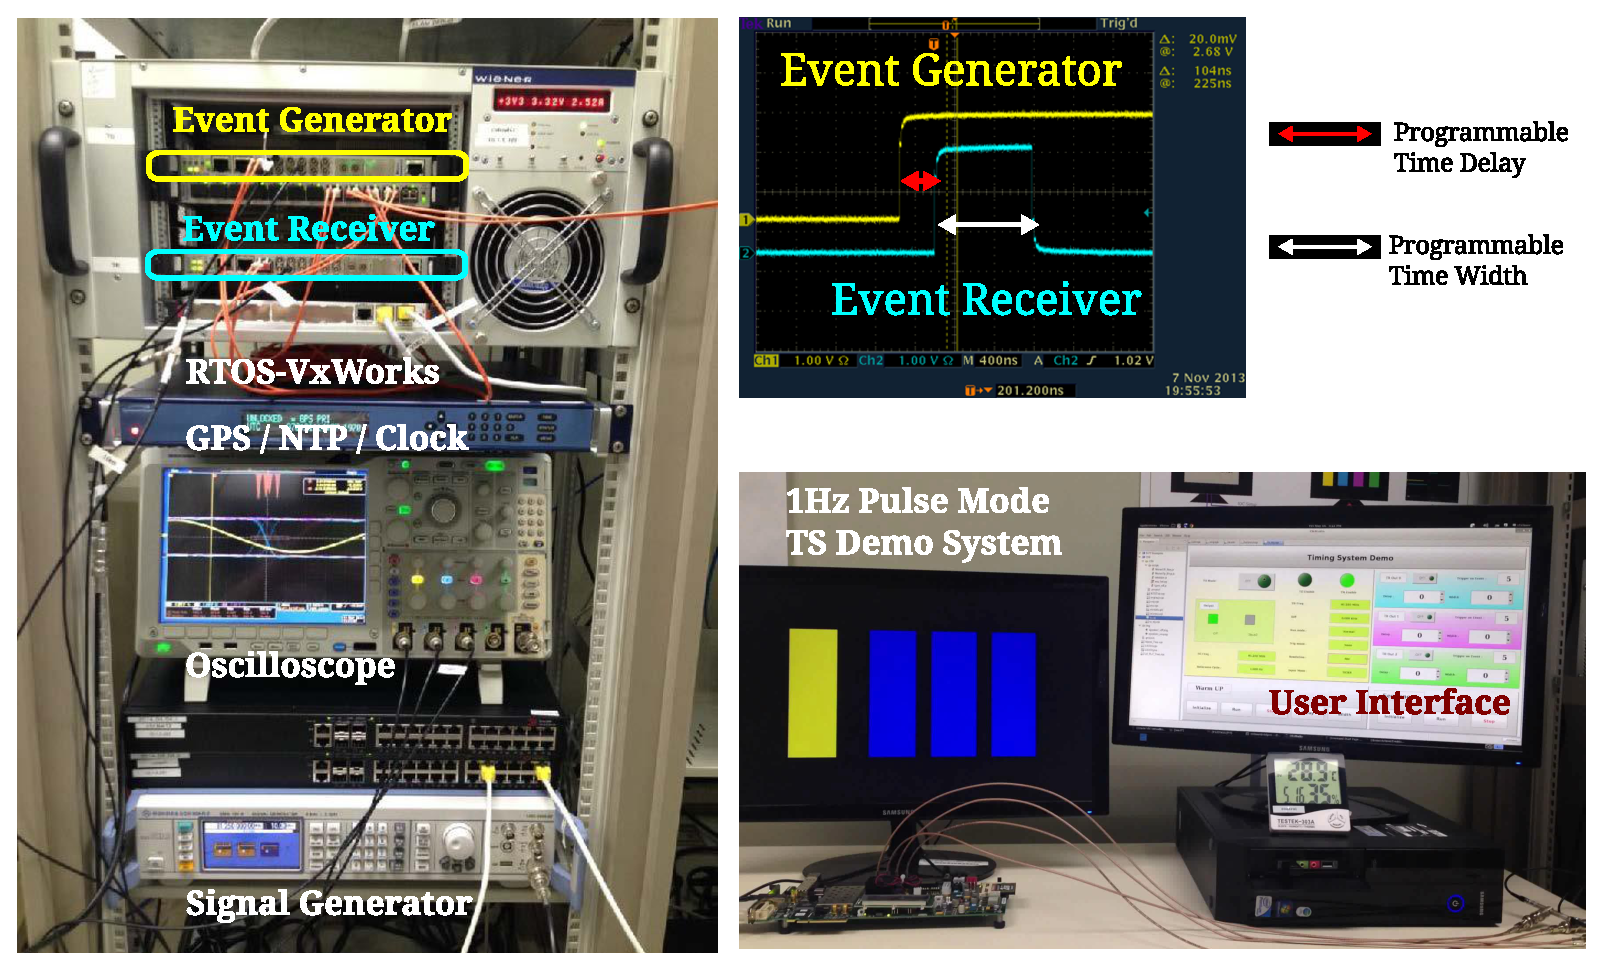
\includegraphics[width=1\columnwidth]{./images/timing_test.eps}
  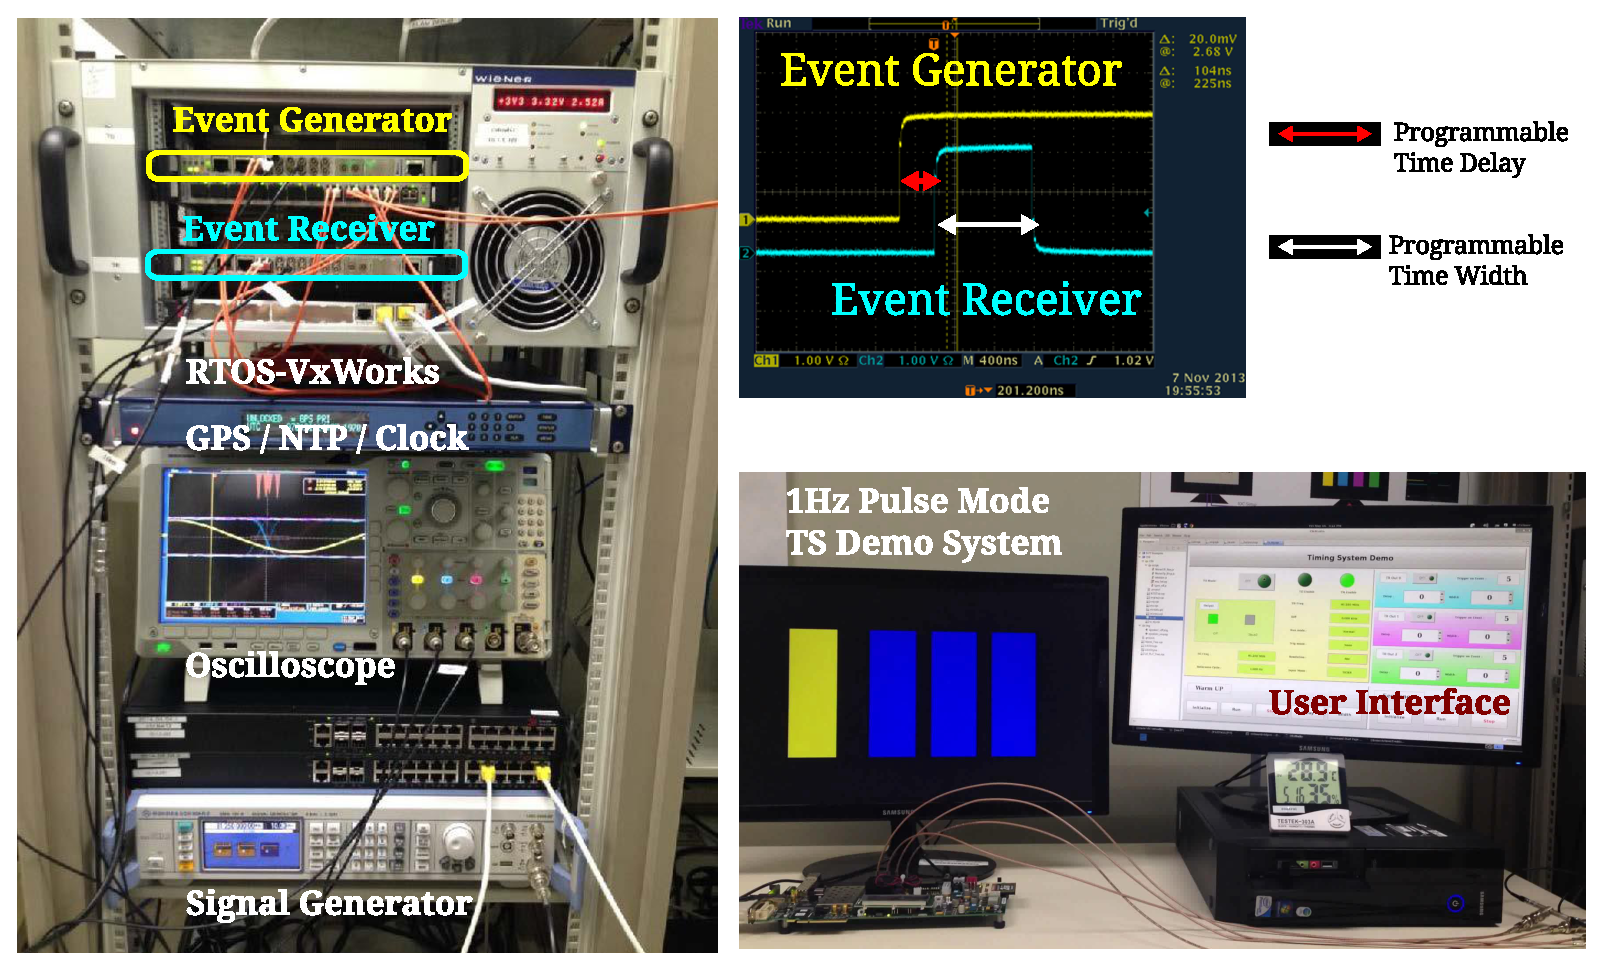
\includegraphics[width=25cm,height=23cm]{./images/timing_test.eps}
 \end{figure}
	  
\begin{itemize}
      \item Hardware Configurations :
   \begin{itemize}
   	\item[-] XLi GPS Time System
   	\item[-] Rubidium Frequency Standard Clock Source (FS725)
   	\item[-] Event Trigger System (EVG/EVR, Fan-out Repeater)
   	\item[-] MVME 6100 / MVME 3100 Controller
   	\item[-] SMA 100a RF Signal Generator
   	\item[-] VME Wiener Crate
   \end{itemize}
   \item Software Configurations :
   \begin{itemize}
   	\item[-] Workbench 3.3, VxWorks IDE
   	\item[-] VxWorks 6.9 Real-time OS (on MVME 6100, EVG)
   	\item[-] RTEMS Real-time OS (on MVME 3100, EVR)
   	\item[-] EPICS framework (R3.14.15.2)
   	\item[-] MRFIOC2 / SRSIOC
   	\item[-] Network Time Protocol (NTP)
   \end{itemize}
   \item Timing Signal Flow :
   \begin{itemize}
	\item GPS receiver synchronizes with RB clock and EVG to 1PPS
	\item Master OSC. generates reference RF (81.25 MHz) to EVG
	\item Two signals of EVG are synchronized by locking phase
	\item Synchronized signal of EVG is generated and distributed to EVR according to event code of MRFIOC2 on VME system
    \end{itemize}
\end{itemize}
\end{mdframed}
\columnbreak
\section*{Fast Controller using Timing Signal}
%\subsection*{Fast Stepper Motor Control Testbed}
\begin{mdframed}[roundcorner=10pt]
	\begin{figure}[H]
		\centering
%		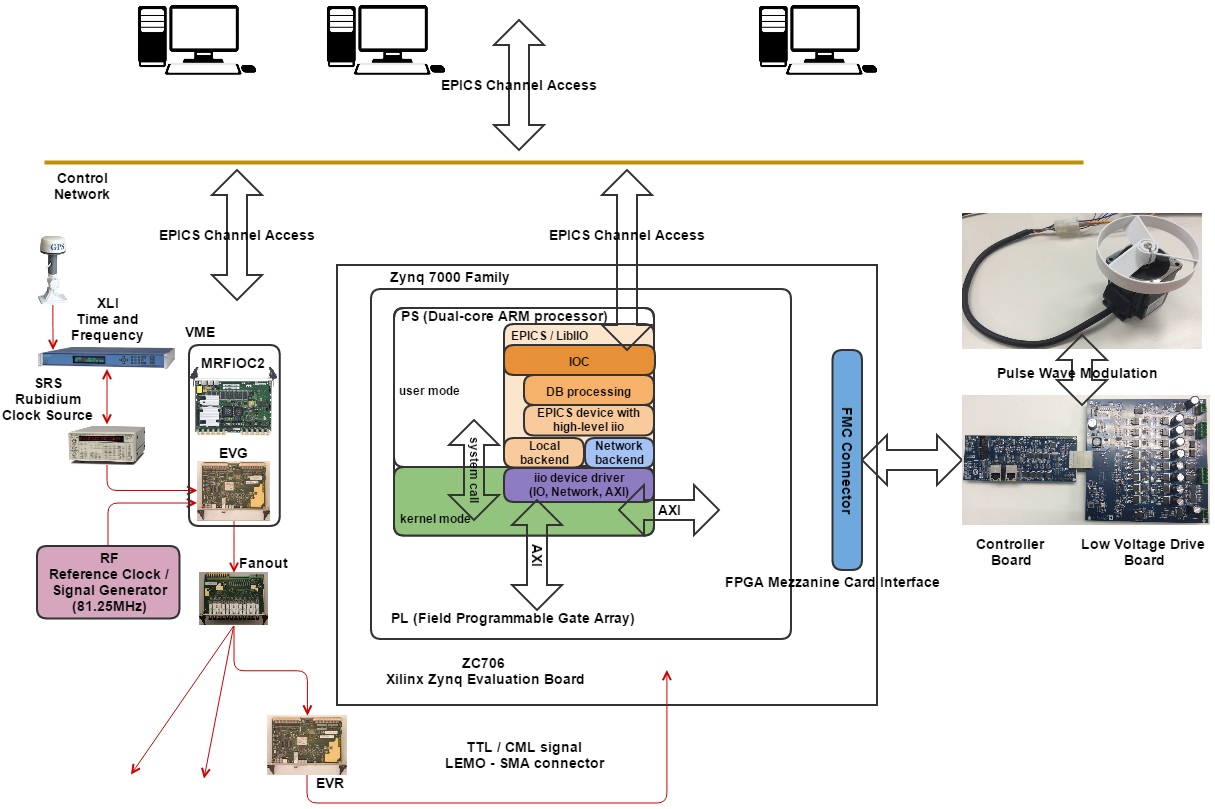
\includegraphics[width=1\textwidth]{./images/WEPGF124f3.eps}
		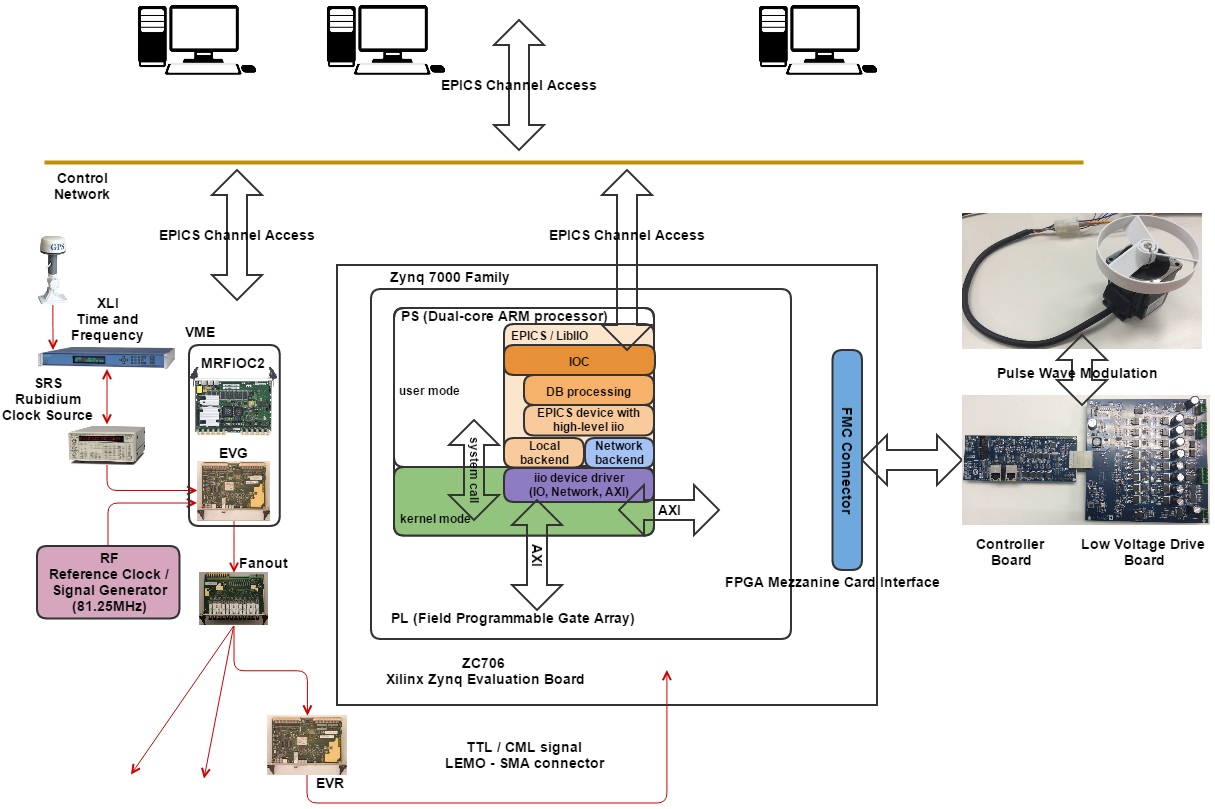
\includegraphics[width=25cm,height=30cm]{./images/WEPGF124f3.eps}
	\end{figure}
\begin{itemize}
  	\item System on Chip: FPGA - Zynq\cite{xilix,zynq}
  	\begin{itemize}
		\item Zynq as SoC is divided into PS and PL
  		\item[-] Interface between PS and PL is through the AXI of AMBA\cite{amba-bus}
  	\end{itemize}
  	\item ZC706 Evaluation Board\cite{zc706-doc}
  	\item Linux on Zynq PS (ARM Processor)
  	\begin{itemize}
  		\item[-] ARM Cross Compile Tool Chain (arm-linuxgnueabihf)
  		\item[-] Linux Kernel Source (Linaro)\cite{linaro}
  		\item[-] Bootloader (BOOT.BIN: FSBL.elf, U-Boot.elf, uImage, Zynq.bif, User.bit)\cite{boot-bin,u-boot}
  		\item[-] Board Support Package (Linux Device Tree)
  		\item[-] Root File System (Busybox)\cite{busybox}
  	\end{itemize}
  	\item Linux Device Driver
  	\begin{itemize}
  		\item[-] Industrial IO linux device driver of Analog Devices\cite{analog}
  		\item[-] Libiio library\cite{iio}
  	\end{itemize}  	
  	\item Software Interface
  	\begin{itemize}
  		\item[-] EPICS Base R3.14.15.2 : IOC developed using Libiio
  		\item[-] FPGA VerilogHDL by Vivado\cite{vivado} (Used the HDL code of Analog Devices)
  	\end{itemize}  	
\end{itemize}
\end{mdframed}

\subsection*{Controller / Low Voltage Drive Board}
\begin{mdframed}[roundcorner=10pt]
\begin{figure}[H]
\centering
  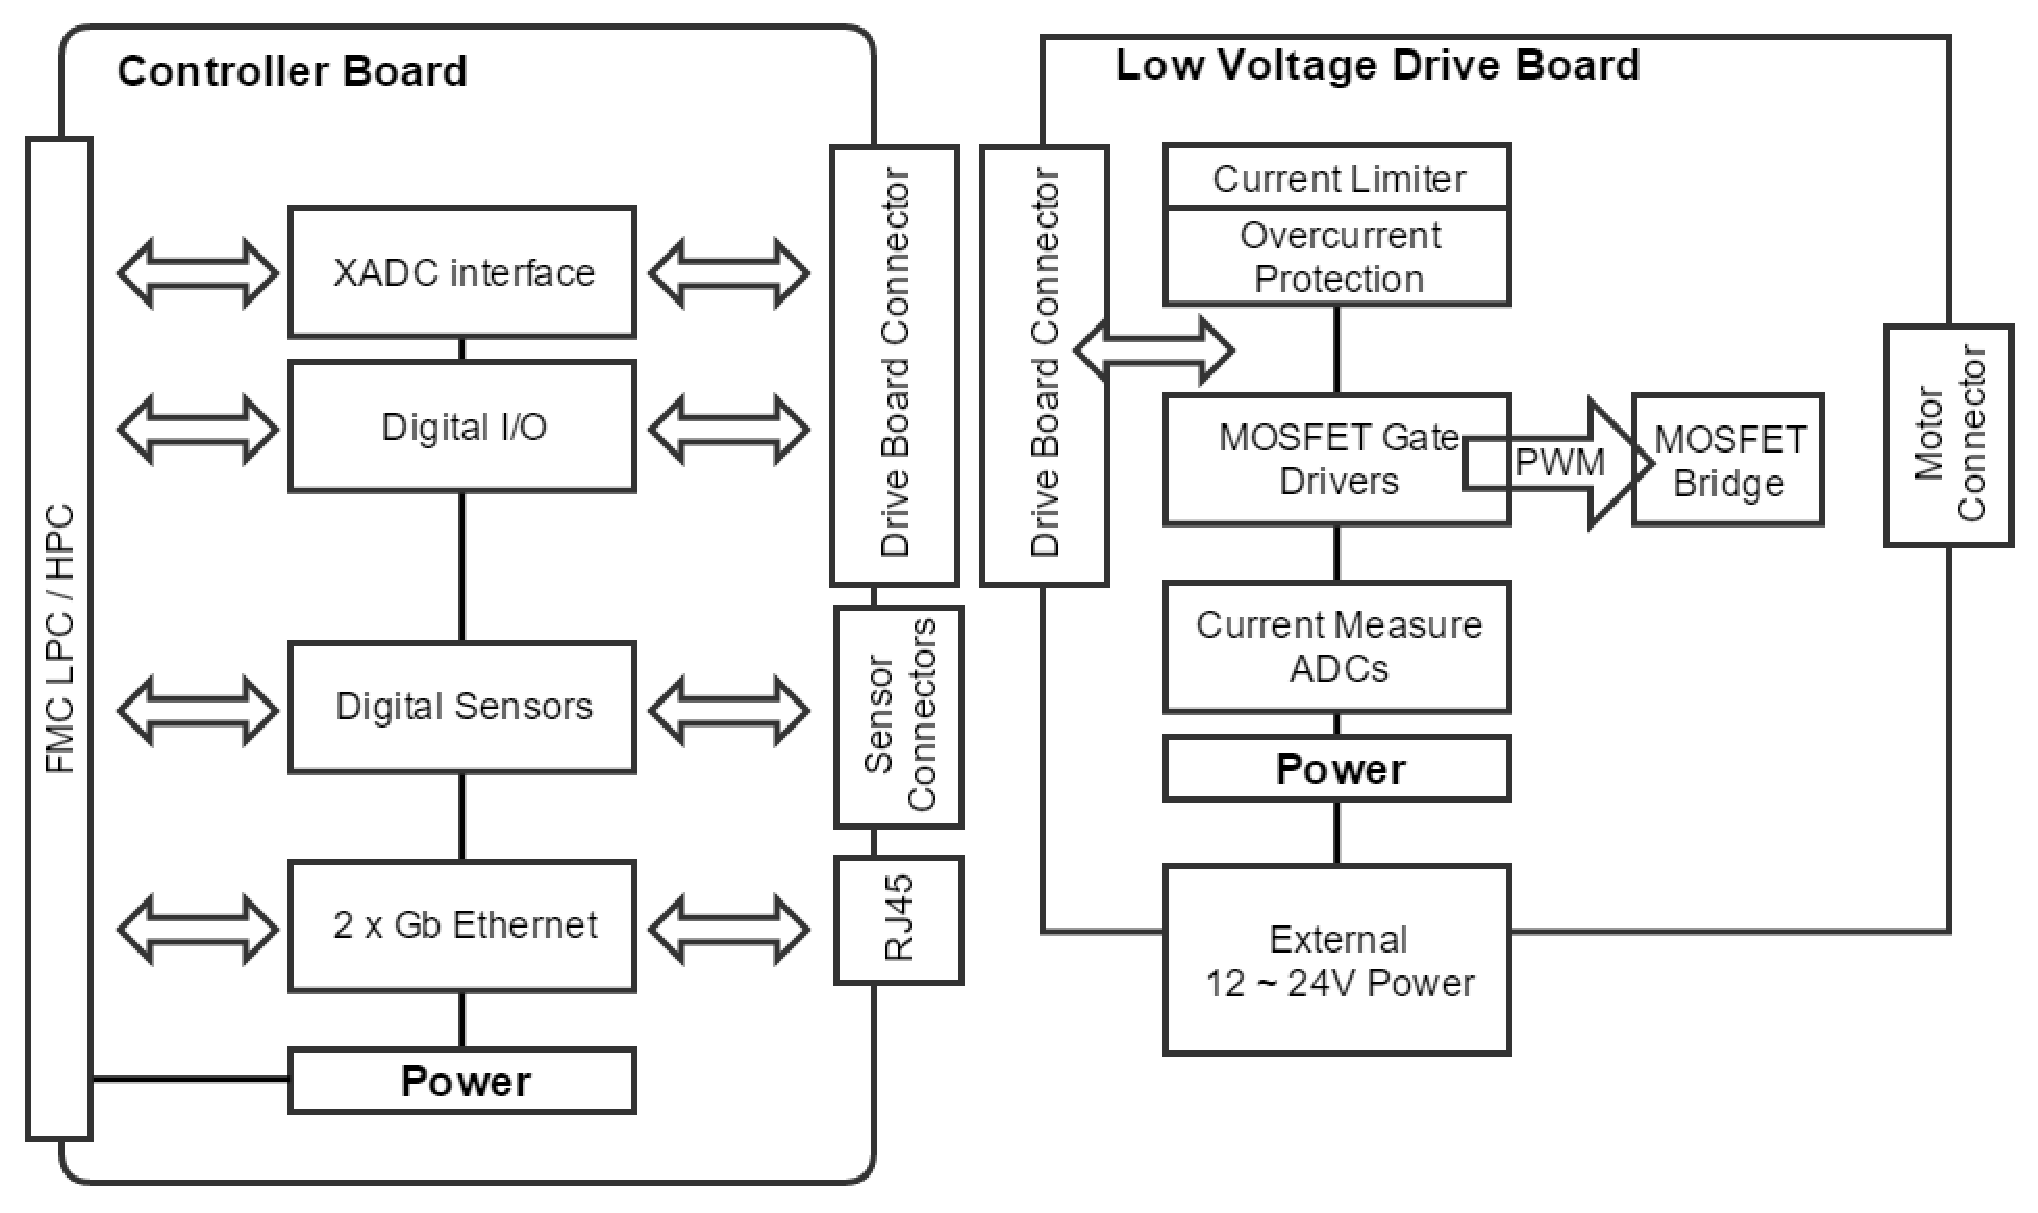
\includegraphics[width=1\columnwidth]{./images/WEPGF124f2.eps}
%\caption{The timing system prototyping}
\label{fig:timing_prototype}
\end{figure}
\begin{itemize}
\item Controller and Low Voltage Drive Board of Analog Devices
\item Controller communicates with ZC706 via FMC Connector
\item FMC Connection: XADC, Digital I/O, 2xGB Ethernet
\item XADC and digital I/O signals to LVDB
\item PWM Signal Generation through MOSFET Gate Drivers
\item External Power: 12 $\sim$24 DC to LVDB
\end{itemize}
\end{mdframed}

\columnbreak

\subsection*{Test Stepper Mortor}
\begin{mdframed}[roundcorner=10pt]
\begin{figure}[H]
	\centering
	\includegraphics[width=25cm,height=15cm]{./images/hw_conf.eps}
\end{figure}
\begin{itemize}
\item Not fully implemented, still is developing FPGA code to receive the timing EVR input signal
\item Left shows to drive stepper motor using EPICS interface
\item Right shows the connection for timing signal between EVR and ZC706
\end{itemize}
\end{mdframed}


\section*{Summary}

\begin{mdframed}[roundcorner=10pt]
	\begin{figure}[H]
		\centering
%		\includegraphics[width=25cm, height=22cm]{./images/conf_table.eps}
		\includegraphics[width=1\textwidth]{./images/conf_table.eps}
	\end{figure}
\end{mdframed}


\section*{Conclusion}
\begin{mdframed}[roundcorner=10pt]
Timing system can distribute the fine synchronized event signal at a high speed. The objective of the stepper motor control testbed is to know how to operate the timing system and how to apply it to the high speed controller. The overall implementation is still underway, however if the distributed control system using EPICS makes a connection with the high speed parallel processing of FPGA, it is possible to improve the performance and efficiency of the control system. Zynq SoC can be considered as an ideal device to implement this high-speed control system.
\end{mdframed}

\section*{Acknowledgement}
This work is supported by the Rare Isotope Science Project funded by 
Ministry of Science, ICT and Future Planning (MSIP) 
and National Research Foundation (NRF) of KOREA.

\begin{thebibliography}{13}   % Use for  1-9  references
%\begin{thebibliography}{99} % Use for 10-99 references

\bibitem{TSHOO:NIMB} Y.~K.~Kwon, {\it et. al},``Status of Rare Isotope Science Project in Korea'', Few-Body Syst 54, 961-966, (2013).

\bibitem{mrf}
Micro-Research Finland Oy: \texttt{http://www.mrf.fi}%


\bibitem{xilix}
Xilinx-FPGA website:
\texttt{http://www.xilinx.com}

\bibitem{zynq}
Zynq-Book Document website:
\texttt{http://www.zynqbook.com}

\bibitem{amba-bus}
Advanced ~Microcontroller ~Bus~ Architecture\\ \texttt{~http://en.wikipedia.org/wiki/\\Advanced\_Microcontroller\_Bus\_Architecture}%

\bibitem{zc706-doc}
ZC706 ~Evaluation ~Board ~Document:\\
\texttt{http://www.xilinx.com/support/documentation/boards\_and\_kits\\/zc706/ug954-zc706-eval-boardxc7z045-ap-soc.pdf}%

\bibitem{linaro}
Linaro Document website:\\
\texttt{https://en.wikipedia.org/wiki/Linaro}


\bibitem{boot-bin}
Boot ~Image ~Document ~website:\\
\texttt{http://www.wiki.xilinx.com/Prepare+boot+image}

\bibitem{u-boot}
U-Boot Document website :
\texttt{http://www.denx.de/wiki/U-Boot}


\bibitem{busybox}
Busybox Document website :
\texttt{http://www.busybox.net/}

\bibitem{analog}
Analog Devices website:
\texttt{http://www.analog.com}

\bibitem{iio}
Industrial ~I/O ~Document ~website:\\
\texttt{https://wiki.analog.com/resources/tools-software\\/linux-software/libiio}


\bibitem{vivado}
Xilinx Vivado Document website:\\
\texttt{http://www.xilinx.com/products/design-tools/vivado.html}

%\bibitem{XAL}
%J. Galambos, {\it et. al.}, ``SNS Application Programming Environment'', EPAC 2002, Paris, France (2002).

%\bibitem{esstechnote0005}
%G. Trahern, ``ESS Naming Convention'', ESS AD Technical Note.
\end{thebibliography}
\end{multicols}
%\vspace{13mm}

%\begin{minipage}[b]{1\linewidth}

%\section*{RAON Major Operations Modes}
%\vspace{2mm}
%\begin{figure}[H]
 % 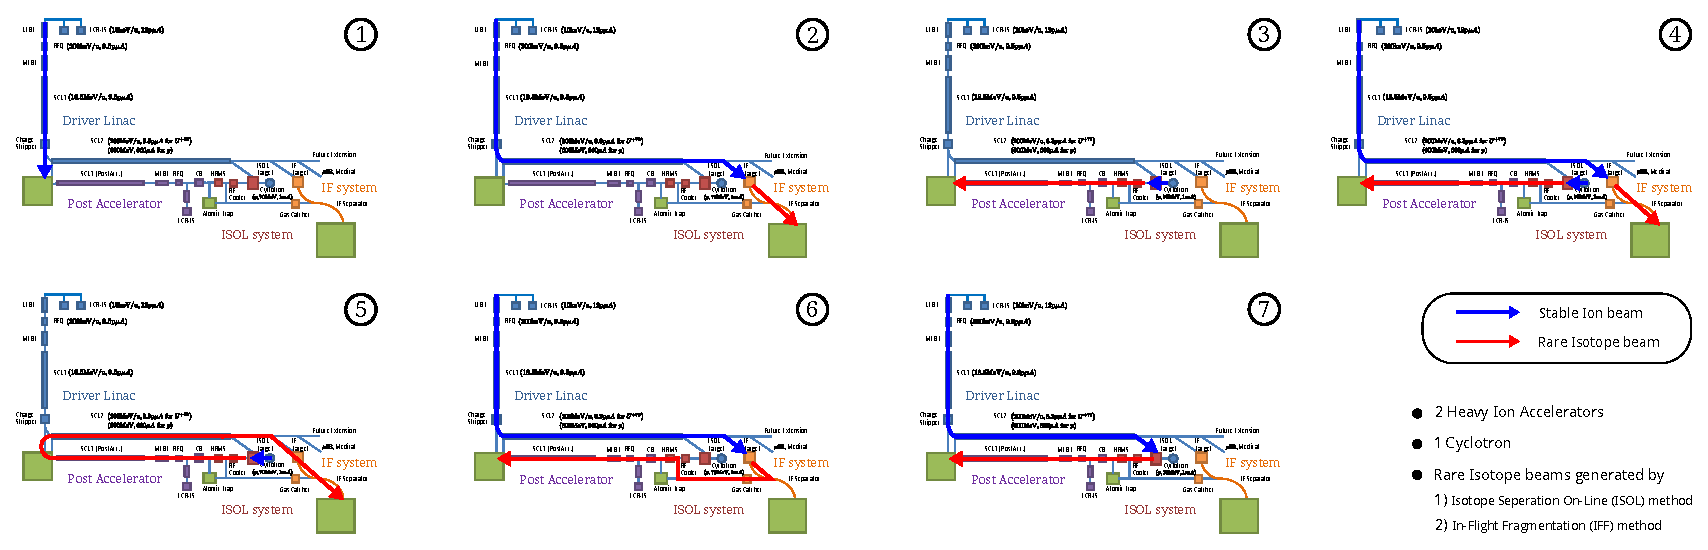
\includegraphics[width=0.99\columnwidth]{./images/raon_all_modes.eps}
%\end{figure}

%\end{minipage}





\end{document}

